\PassOptionsToPackage{unicode=true}{hyperref} % options for packages loaded elsewhere
\PassOptionsToPackage{hyphens}{url}
%
\documentclass[10pt,xcolor=table,color={dvipsnames,usenames},ignorenonframetext,usepdftitle=false,french]{beamer}
\setbeamertemplate{caption}[numbered]
\setbeamertemplate{caption label separator}{: }
\setbeamercolor{caption name}{fg=normal text.fg}
\beamertemplatenavigationsymbolsempty
\usepackage{caption}
\captionsetup{skip=0pt,belowskip=0pt}
%\setlength\abovecaptionskip{-15pt}
\usepackage{lmodern}
\usepackage{amssymb,amsmath,mathtools,multirow}
\usepackage{float,hhline}
\usepackage{tikz}
\usepackage[tikz]{bclogo}
\usepackage{mathtools}
\usepackage{ifxetex,ifluatex}
\usepackage{fixltx2e} % provides \textsubscript
\ifnum 0\ifxetex 1\fi\ifluatex 1\fi=0 % if pdftex
  \usepackage[T1]{fontenc}
  \usepackage[utf8]{inputenc}
  \usepackage{textcomp} % provides euro and other symbols
\else % if luatex or xelatex
  \usepackage{unicode-math}
  \defaultfontfeatures{Ligatures=TeX,Scale=MatchLowercase}
\fi
\usetheme[coding=utf8,language=english,
,titlepagelogo=img/SACElogo.jpg
]{TorinoTh}
% use upquote if available, for straight quotes in verbatim environments
\IfFileExists{upquote.sty}{\usepackage{upquote}}{}
% use microtype if available
\IfFileExists{microtype.sty}{%
\usepackage[]{microtype}
\UseMicrotypeSet[protrusion]{basicmath} % disable protrusion for tt fonts
}{}
\IfFileExists{parskip.sty}{%
\usepackage{parskip}
}{% else
\setlength{\parindent}{0pt}
\setlength{\parskip}{6pt plus 2pt minus 1pt}
}
\usepackage{hyperref}
\hypersetup{
            pdftitle={RJDemetra: an R interface to JDemetra+},
            pdfauthor={Alain Quartier-la-Tente and Anna Michalek},
            pdfborder={0 0 0},
            breaklinks=true}
\urlstyle{same}  % don't use monospace font for urls
\newif\ifbibliography
\usepackage{color}
\usepackage{fancyvrb}
\newcommand{\VerbBar}{|}
\newcommand{\VERB}{\Verb[commandchars=\\\{\}]}
\DefineVerbatimEnvironment{Highlighting}{Verbatim}{commandchars=\\\{\}}
% Add ',fontsize=\small' for more characters per line
\usepackage{framed}
\definecolor{shadecolor}{RGB}{248,248,248}
\newenvironment{Shaded}{\begin{snugshade}}{\end{snugshade}}
\newcommand{\AlertTok}[1]{\textcolor[rgb]{0.94,0.16,0.16}{#1}}
\newcommand{\AnnotationTok}[1]{\textcolor[rgb]{0.56,0.35,0.01}{\textbf{\textit{#1}}}}
\newcommand{\AttributeTok}[1]{\textcolor[rgb]{0.77,0.63,0.00}{#1}}
\newcommand{\BaseNTok}[1]{\textcolor[rgb]{0.00,0.00,0.81}{#1}}
\newcommand{\BuiltInTok}[1]{#1}
\newcommand{\CharTok}[1]{\textcolor[rgb]{0.31,0.60,0.02}{#1}}
\newcommand{\CommentTok}[1]{\textcolor[rgb]{0.56,0.35,0.01}{\textit{#1}}}
\newcommand{\CommentVarTok}[1]{\textcolor[rgb]{0.56,0.35,0.01}{\textbf{\textit{#1}}}}
\newcommand{\ConstantTok}[1]{\textcolor[rgb]{0.00,0.00,0.00}{#1}}
\newcommand{\ControlFlowTok}[1]{\textcolor[rgb]{0.13,0.29,0.53}{\textbf{#1}}}
\newcommand{\DataTypeTok}[1]{\textcolor[rgb]{0.13,0.29,0.53}{#1}}
\newcommand{\DecValTok}[1]{\textcolor[rgb]{0.00,0.00,0.81}{#1}}
\newcommand{\DocumentationTok}[1]{\textcolor[rgb]{0.56,0.35,0.01}{\textbf{\textit{#1}}}}
\newcommand{\ErrorTok}[1]{\textcolor[rgb]{0.64,0.00,0.00}{\textbf{#1}}}
\newcommand{\ExtensionTok}[1]{#1}
\newcommand{\FloatTok}[1]{\textcolor[rgb]{0.00,0.00,0.81}{#1}}
\newcommand{\FunctionTok}[1]{\textcolor[rgb]{0.00,0.00,0.00}{#1}}
\newcommand{\ImportTok}[1]{#1}
\newcommand{\InformationTok}[1]{\textcolor[rgb]{0.56,0.35,0.01}{\textbf{\textit{#1}}}}
\newcommand{\KeywordTok}[1]{\textcolor[rgb]{0.13,0.29,0.53}{\textbf{#1}}}
\newcommand{\NormalTok}[1]{#1}
\newcommand{\OperatorTok}[1]{\textcolor[rgb]{0.81,0.36,0.00}{\textbf{#1}}}
\newcommand{\OtherTok}[1]{\textcolor[rgb]{0.56,0.35,0.01}{#1}}
\newcommand{\PreprocessorTok}[1]{\textcolor[rgb]{0.56,0.35,0.01}{\textit{#1}}}
\newcommand{\RegionMarkerTok}[1]{#1}
\newcommand{\SpecialCharTok}[1]{\textcolor[rgb]{0.00,0.00,0.00}{#1}}
\newcommand{\SpecialStringTok}[1]{\textcolor[rgb]{0.31,0.60,0.02}{#1}}
\newcommand{\StringTok}[1]{\textcolor[rgb]{0.31,0.60,0.02}{#1}}
\newcommand{\VariableTok}[1]{\textcolor[rgb]{0.00,0.00,0.00}{#1}}
\newcommand{\VerbatimStringTok}[1]{\textcolor[rgb]{0.31,0.60,0.02}{#1}}
\newcommand{\WarningTok}[1]{\textcolor[rgb]{0.56,0.35,0.01}{\textbf{\textit{#1}}}}
\usepackage{graphicx,grffile}
\makeatletter
\def\maxwidth{\ifdim\Gin@nat@width>\linewidth\linewidth\else\Gin@nat@width\fi}
\def\maxheight{\ifdim\Gin@nat@height>\textheight\textheight\else\Gin@nat@height\fi}
\makeatother
% Scale images if necessary, so that they will not overflow the page
% margins by default, and it is still possible to overwrite the defaults
% using explicit options in \includegraphics[width, height, ...]{}
\setkeys{Gin}{width=\maxwidth,height=\maxheight,keepaspectratio}
% Prevent slide breaks in the middle of a paragraph:
\widowpenalties 1 10000
\raggedbottom
\AtBeginPart{
  \let\insertpartnumber\relax
  \let\partname\relax
  \frame{\partpage}
}
\AtBeginSection{
  \ifbibliography
  \else
    \begin{frame}{Sommaire}
    \tableofcontents[currentsection, hideothersubsections]
    \end{frame}
  \fi
}
\setlength{\emergencystretch}{3em}  % prevent overfull lines
\providecommand{\tightlist}{%
  %\setlength{\itemsep}{0pt}
  \setlength{\parskip}{0pt}
  }
\setcounter{secnumdepth}{0}

% set default figure placement to htbp
\makeatletter
\def\fps@figure{htbp}
\makeatother

\usepackage{booktabs}
\usepackage{longtable}
\usepackage{array}
\usepackage{multirow}
\usepackage[table]{xcolor}
\usepackage{wrapfig}
\usepackage{float}
\usepackage{colortbl}
\usepackage{pdflscape}
\usepackage{tabu}
\usepackage{threeparttable}
\usepackage{threeparttablex}
\usepackage[normalem]{ulem}
\usepackage{makecell}
\usepackage{animate}

\title{RJDemetra: an R interface to JDemetra+}
\ateneo{NTTS, 13 March 2019}
\author{Alain Quartier-la-Tente and Anna Michalek}
\date{}


\setrellabel{}

\setcandidatelabel{}

\rel{}
\division{Insee, Seasonal Adjustment Centre of Excellence (AQLT) and European
Central Bank (AM)}

\departement{}
\makeatletter
\let\@@magyar@captionfix\relax
\makeatother

\DeclareMathOperator{\Cov}{Cov}
\newcommand{\E}[1]{\mathbb{E}\left[ #1 \right]}
\newcommand{\V}[1]{\mathbb{V}\left[ #1 \right]}
\newcommand{\cov}[2]{\Cov\left( #1\,,\,#2 \right)}

\begin{document}
\begin{frame}[plain,noframenumbering]
\titlepage
\end{frame}

\hypertarget{rjdemetra}{%
\section{RJDemetra}\label{rjdemetra}}

\hypertarget{purpose-and-current-status}{%
\subsection{Purpose and current
status}\label{purpose-and-current-status}}

\begin{frame}{Purpose of the RJDemetra package}
\protect\hypertarget{purpose-of-the-rjdemetra-package}{}

\begin{itemize}
\tightlist
\item
  Complete R package for Tramo-Seats and X13\\
\item
  Users: ``pure R'' package

  \begin{itemize}
  \tightlist
  \item
    Part of R routines, automatization

    \begin{itemize}
    \tightlist
    \item
      Batch processing
    \item
      E.g.: direct vs indirect aggregates adjustment, dashboards
    \end{itemize}
  \item
    Usage of other R functions and packages
  \end{itemize}
\item
  JD+ functionality

  \begin{itemize}
  \tightlist
  \item
    Modeling and seasonal adjustment
  \item
    Full specification
  \end{itemize}
\item
  Advanced graphical presentation: JD+
\end{itemize}

\end{frame}

\begin{frame}{Current status}
\protect\hypertarget{current-status}{}

\begin{itemize}
\tightlist
\item
  RegARIMA, TRAMO-SEATS and X-13-ARIMA:

  \begin{itemize}
  \tightlist
  \item
    R package with documentation\\
  \item
    S3 classes with plot, summary, print methods
  \item
    Possibility to add user-defined regressors but not user-defined
    calendar regressors
  \end{itemize}
\item
  Manipulate workspace (only TRAMO-SEATS and X-13-ARIMA):

  \begin{itemize}
  \tightlist
  \item
    Import JD+ workspace to get: input raw series or SA model
  \item
    Export R models created via RJDemetra
  \end{itemize}
\end{itemize}

├─ \textbar{}- = = ---\textbar{} └─

\end{frame}

\hypertarget{some-examples}{%
\section{Some examples}\label{some-examples}}

\hypertarget{regarima-examples}{%
\subsection{RegARIMA examples}\label{regarima-examples}}

\begin{frame}[fragile]{RegARIMA examples (1/4)}
\protect\hypertarget{regarima-examples-14}{}

\footnotesize

\begin{Shaded}
\begin{Highlighting}[]
\KeywordTok{library}\NormalTok{(RJDemetra);}\KeywordTok{options}\NormalTok{(}\DataTypeTok{enable_print_style =} \OtherTok{FALSE}\NormalTok{)}
\NormalTok{myseries <-}\StringTok{ }\NormalTok{ipi_c_eu[,}\StringTok{"FR"}\NormalTok{]}
\NormalTok{regarima_model <-}\StringTok{ }\KeywordTok{regarima_def_x13}\NormalTok{(myseries, }\DataTypeTok{spec =} \StringTok{"RG4c"}\NormalTok{)}
\KeywordTok{str}\NormalTok{(regarima_model, }\DataTypeTok{max.level =} \DecValTok{1}\NormalTok{)}
\end{Highlighting}
\end{Shaded}

\begin{verbatim}
## List of 9
##  $ specification          :List of 7
##  $ arma                   : Named num [1:6] 2 1 1 0 1 1
##   ..- attr(*, "names")= chr [1:6] "p" "d" "q" "bp" ...
##  $ arima.coefficients     : num [1:4, 1:3] 0.336 0.206 -0.245 -0.511 0.171 ...
##   ..- attr(*, "dimnames")=List of 2
##  $ regression.coefficients: num [1:4, 1:3] -1.133 -8 -7.551 -5.069 0.337 ...
##   ..- attr(*, "dimnames")=List of 2
##  $ loglik                 : num [1:7, 1] -631 9 323 1280 1281 ...
##   ..- attr(*, "dimnames")=List of 2
##  $ model                  :List of 2
##  $ residuals              : Time-Series [1:323] from 1991 to 2018: -2.601 0.573 -1.776 -1.374 2.155 ...
##  $ residuals.stat         :List of 2
##  $ forecast               : Time-Series [1:24, 1:2] from 2018 to 2020: 102 103 114 109 103 ...
##   ..- attr(*, "dimnames")=List of 2
##  - attr(*, "class")= chr [1:2] "regarima" "X13"
\end{verbatim}

\end{frame}

\begin{frame}{RegARIMA examples (2/4)}
\protect\hypertarget{regarima-examples-24}{}

\animategraphics[loop, autoplay, width=\linewidth]{4}{img/gif/regarima_print/img_}{1}{37}

\end{frame}

\begin{frame}[fragile]{RegARIMA examples (3/4)}
\protect\hypertarget{regarima-examples-34}{}

\begin{Shaded}
\begin{Highlighting}[]
\KeywordTok{layout}\NormalTok{(}\KeywordTok{matrix}\NormalTok{(}\DecValTok{1}\OperatorTok{:}\DecValTok{6}\NormalTok{, }\DecValTok{3}\NormalTok{, }\DecValTok{2}\NormalTok{));}\KeywordTok{plot}\NormalTok{(regarima_model, }\DataTypeTok{ask =} \OtherTok{FALSE}\NormalTok{)}
\end{Highlighting}
\end{Shaded}

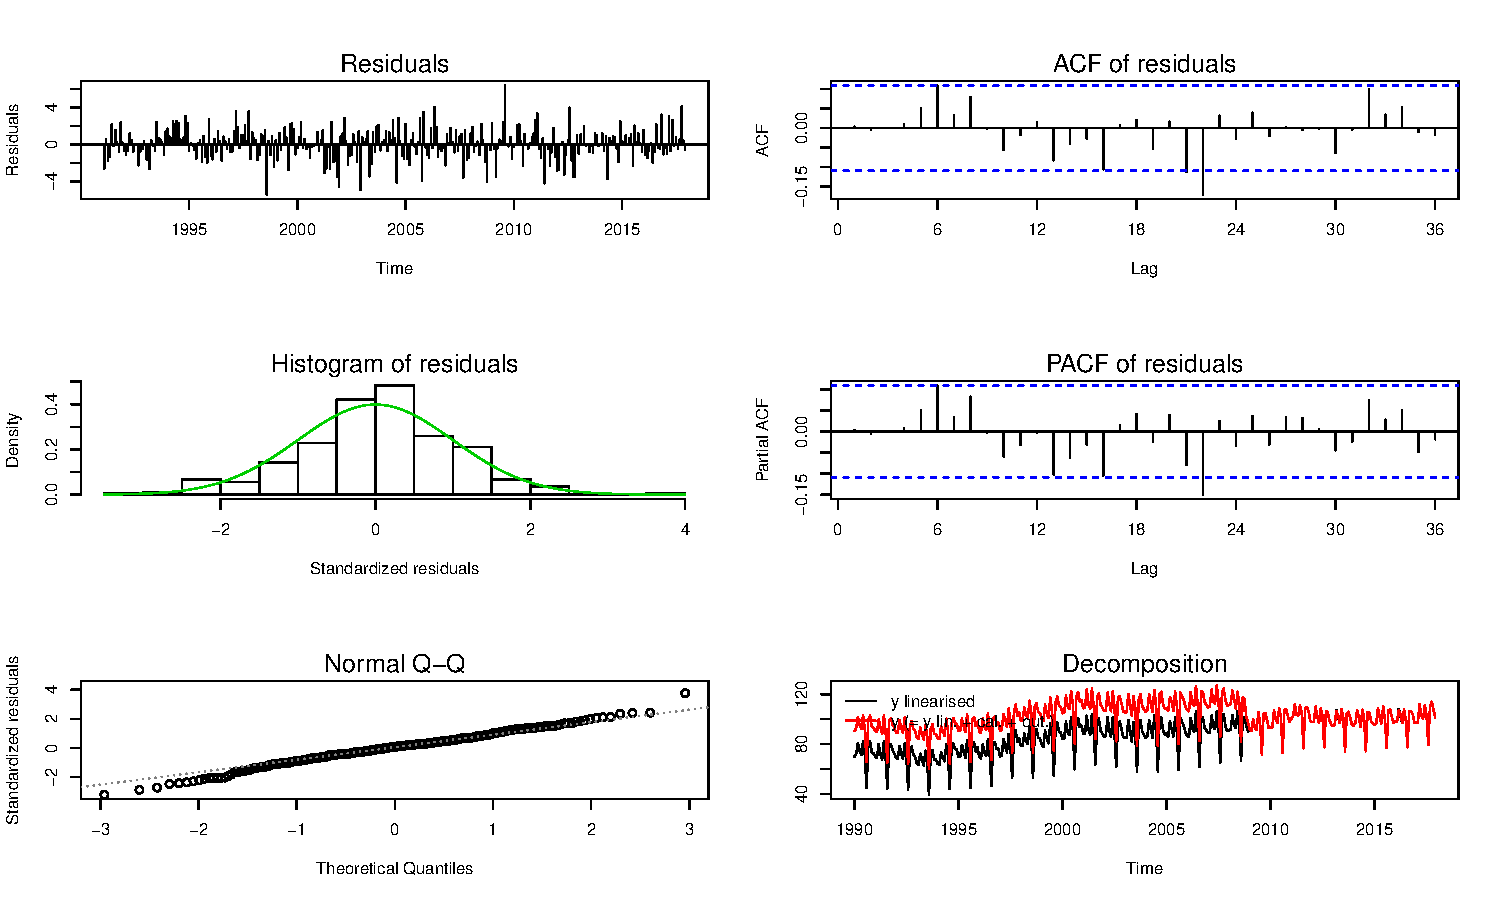
\includegraphics{img/markdown-unnamed-chunk-3-1.pdf}

\end{frame}

\begin{frame}[fragile]{RegARIMA examples (3/4): extra plot}
\protect\hypertarget{regarima-examples-34-extra-plot}{}

\footnotesize

\begin{Shaded}
\begin{Highlighting}[]
\KeywordTok{plot}\NormalTok{(regarima_model, }\DataTypeTok{which =} \DecValTok{7}\NormalTok{, }\DataTypeTok{dec_zoom =} \OtherTok{TRUE}\NormalTok{)}
\end{Highlighting}
\end{Shaded}

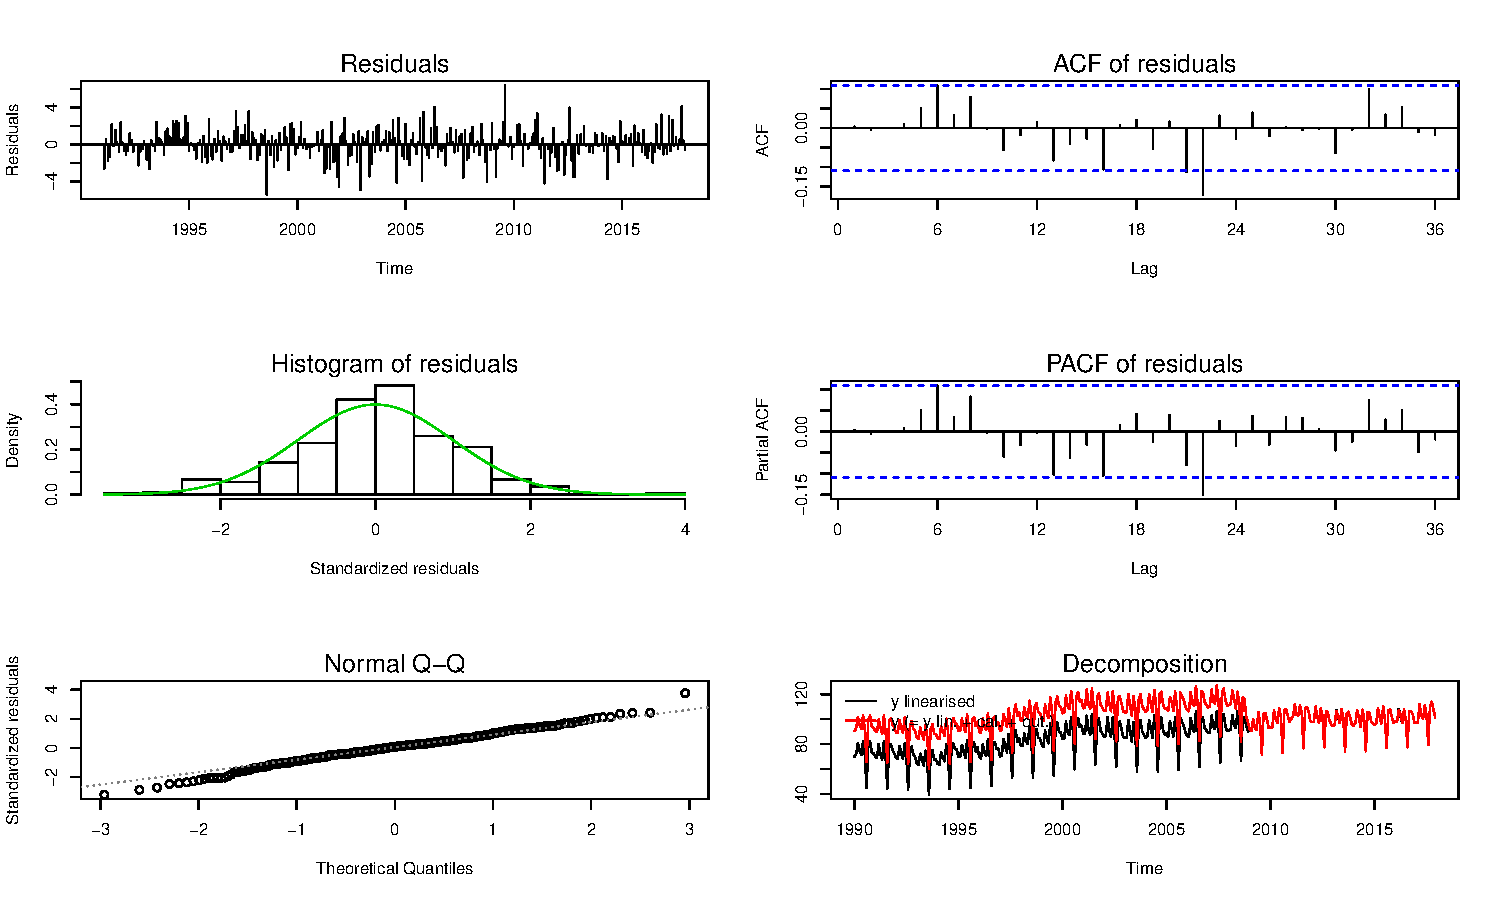
\includegraphics{img/markdown-unnamed-chunk-5-1.pdf}

\end{frame}

\hypertarget{seasonal-adjustment-examples}{%
\subsection{Seasonal adjustment
examples}\label{seasonal-adjustment-examples}}

\begin{frame}[fragile]{Seasonal adjustment examples (1/7)}
\protect\hypertarget{seasonal-adjustment-examples-17}{}

A \texttt{SA} object is a \texttt{list()} of 5 elements:

\begin{enumerate}
\tightlist
\item
  \texttt{regarima}: the RegArima model
\item
  \texttt{decomposition}: decomposition variables (\(\ne\) for
  TRAMO-SEATS and X-13-ARIMA)
\item
  \texttt{final}: time series main results
\item
  \texttt{diagnostics}: residuals tests, etc.
\item
  \texttt{user\_defined}: other user\_defined variables not exported by
  default (see \texttt{?user\_defined\_variables})
\end{enumerate}

\footnotesize

\begin{Shaded}
\begin{Highlighting}[]
\NormalTok{x13_usr_spec <-}\StringTok{ }\KeywordTok{x13_spec_def}\NormalTok{(}\DataTypeTok{spec=}\KeywordTok{c}\NormalTok{(}\StringTok{"RSA5c"}\NormalTok{),}\DataTypeTok{usrdef.outliersEnabled =} \OtherTok{TRUE}\NormalTok{,}
                             \DataTypeTok{usrdef.outliersType =} \KeywordTok{c}\NormalTok{(}\StringTok{"LS"}\NormalTok{,}\StringTok{"AO"}\NormalTok{),}
                             \DataTypeTok{usrdef.outliersDate=}\KeywordTok{c}\NormalTok{(}\StringTok{"2008-10-01"}\NormalTok{,}\StringTok{"2002-01-01"}\NormalTok{),}
                             \DataTypeTok{usrdef.outliersCoef =} \KeywordTok{c}\NormalTok{(}\DecValTok{36000}\NormalTok{,}\DecValTok{14000}\NormalTok{),}
                             \DataTypeTok{transform.function =} \StringTok{"None"}\NormalTok{)}
\NormalTok{x13_mod <-}\StringTok{ }\KeywordTok{x13}\NormalTok{(myseries, x13_usr_spec)}
\NormalTok{ts_mod <-}\StringTok{ }\KeywordTok{tramoseats_def}\NormalTok{(myseries, }\DataTypeTok{spec =} \StringTok{"RSAfull"}\NormalTok{)}
\end{Highlighting}
\end{Shaded}

\end{frame}

\begin{frame}[fragile]{Seasonal adjustment examples (2/7)}
\protect\hypertarget{seasonal-adjustment-examples-27}{}

\footnotesize

\begin{Shaded}
\begin{Highlighting}[]
\NormalTok{x13_mod}\OperatorTok{$}\NormalTok{decomposition}
\end{Highlighting}
\end{Shaded}

\begin{verbatim}
##  Monitoring and Quality Assessment Statistics:  
##       M stats
## M(1)    0.061
## M(2)    0.000
## M(3)    0.960
## M(4)    0.621
## M(5)    0.725
## M(6)    0.244
## M(7)    0.075
## M(8)    0.216
## M(9)    0.055
## M(10)   0.175
## M(11)   0.160
## Q       0.302
## Q-M2    0.339
## 
## Final filters: 
## Seasonal filter:  3x5
## Trend filter:  13 terms Henderson moving average
\end{verbatim}

\end{frame}

\begin{frame}[fragile]{Seasonal adjustment examples (3/7)}
\protect\hypertarget{seasonal-adjustment-examples-37}{}

\footnotesize

\begin{Shaded}
\begin{Highlighting}[]
\NormalTok{ts_mod}\OperatorTok{$}\NormalTok{decomposition}
\end{Highlighting}
\end{Shaded}

\begin{verbatim}
## Model
## AR :  1 + 0.352498 B + 0.133616 B^2 
## D :  1 - B - B^12 + B^13 
## MA :  1 - 0.186819 B - 0.610856 B^12 + 0.114119 B^13 
## 
## 
## SA
## D :  1 - 2.000000 B + B^2 
## MA :  1 - 1.314459 B + 0.340427 B^2 
## Innovation variance:  0.4669153 
## 
## Trend
## D :  1 - 2.000000 B + B^2 
## MA :  1 + 0.040206 B - 0.959794 B^2 
## Innovation variance:  0.04869563 
## 
## Seasonal
## AR :  1 + 0.352498 B + 0.133616 B^2 
## D :  1 + B + B^2 + B^3 + B^4 + B^5 + B^6 + B^7 + B^8 + B^9 + B^10 + B^11 
## MA :  1 + 0.717848 B + 0.460721 B^2 + 0.310085 B^3 + 0.132447 B^4 - 0.049053 B^5 - 0.216655 B^6 - 0.354556 B^7 - 0.445030 B^8 - 0.469587 B^9 - 0.376625 B^10 - 0.166397 B^11 - 0.410618 B^12 - 0.132580 B^13 
## Innovation variance:  0.1601924 
## 
## Irregular
## Innovation variance:  0.2056884
\end{verbatim}

\end{frame}

\begin{frame}[fragile]{Seasonal adjustment examples (4/7)}
\protect\hypertarget{seasonal-adjustment-examples-47}{}

\begin{Shaded}
\begin{Highlighting}[]
\KeywordTok{plot}\NormalTok{(x13_mod}\OperatorTok{$}\NormalTok{decomposition)}
\end{Highlighting}
\end{Shaded}

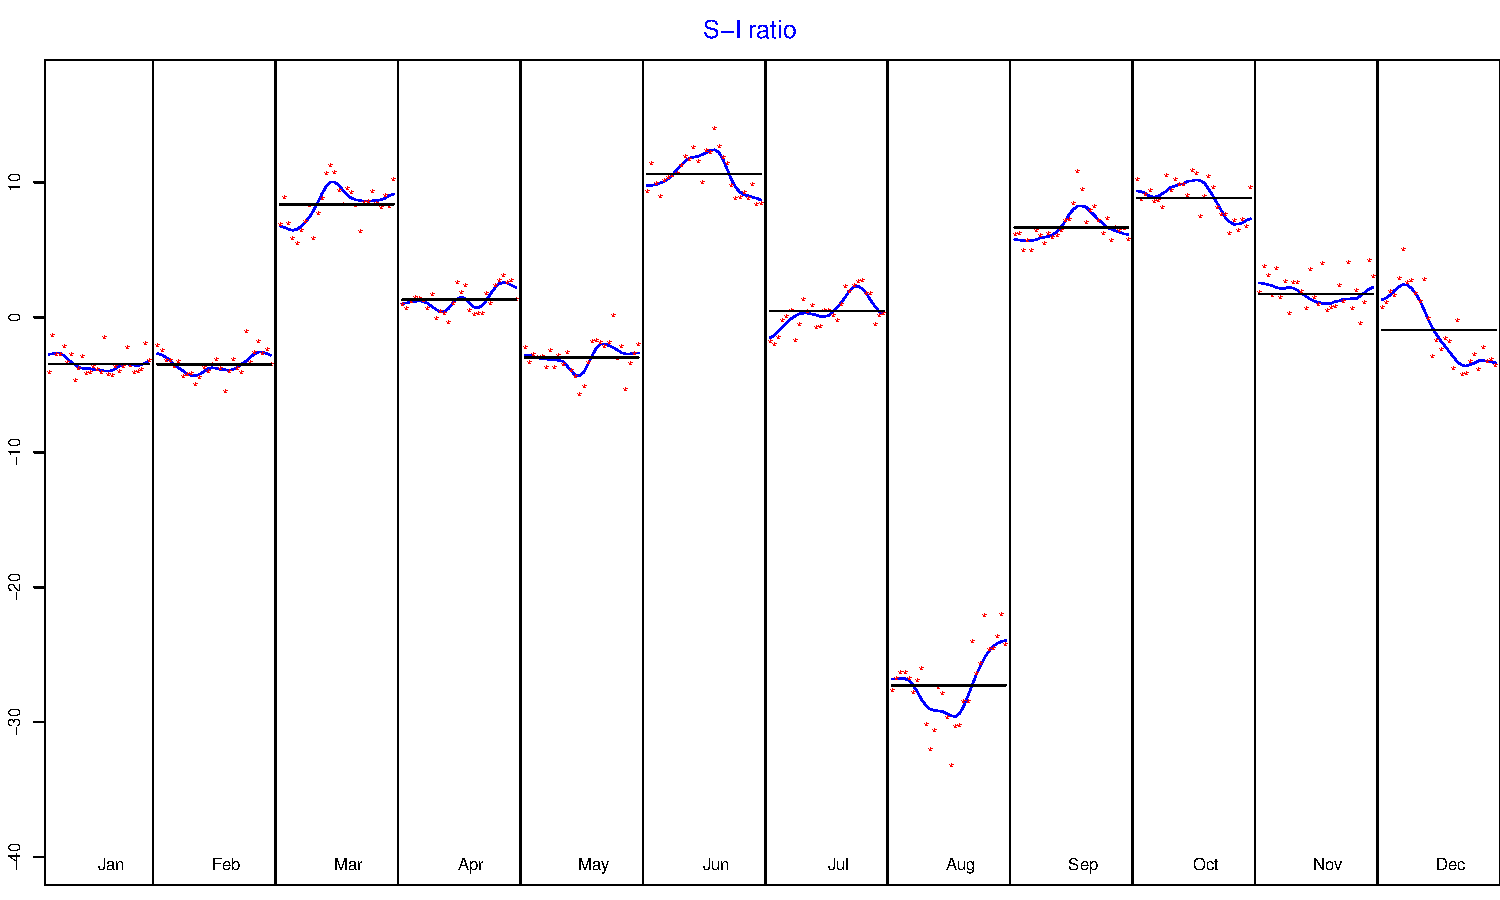
\includegraphics{img/markdown-unnamed-chunk-9-1.pdf}

\end{frame}

\begin{frame}[fragile]{Seasonal adjustment examples (5/7)}
\protect\hypertarget{seasonal-adjustment-examples-57}{}

\footnotesize

\begin{Shaded}
\begin{Highlighting}[]
\NormalTok{x13_mod}\OperatorTok{$}\NormalTok{final}
\end{Highlighting}
\end{Shaded}

\begin{verbatim}
## Last observed values
##              y       sa        t            s          i
## Jan 2017  97.4 100.3902 100.5631  -2.99019403 -0.1729099
## Feb 2017  97.5 100.3646 100.9790  -2.86460513 -0.6143814
## Mar 2017 112.0 102.7607 101.4754   9.23928088  1.2852852
## Apr 2017 103.0 100.5925 101.9417   2.40747193 -1.3491871
## May 2017 100.4 103.1054 102.3511  -2.70539979  0.7542873
## Jun 2017 111.2 102.5591 102.7440   8.64087923 -0.1848857
## Jul 2017 103.4 103.3144 103.1308   0.08560672  0.1835989
## Aug 2017  79.3 103.0602 103.5499 -23.76018864 -0.4897563
## Sep 2017 109.7 103.6331 104.0215   6.06692870 -0.3884680
## Oct 2017 114.0 106.7526 104.5113   7.24741395  2.2412439
## Nov 2017 107.7 105.5963 104.9317   2.10371268  0.6645400
## Dec 2017 101.4 104.8511 105.2567  -3.45110589 -0.4056223
## 
## Forecasts:
##                y_f     sa_f      t_f          s_f         i_f
## Jan 2018 102.70258 105.5740 105.4465  -2.87143758  0.12749286
## Feb 2018 102.57727 105.5466 105.5700  -2.96928512 -0.02343246
## Mar 2018 114.89223 105.6137 105.6941   9.27854825 -0.08039957
## Apr 2018 108.05979 105.6858 105.8691   2.37398629 -0.18326092
## May 2018 103.52705 106.1896 106.1079  -2.66254960  0.08166967
## Jun 2018 114.95898 106.4105 106.3950   8.54848111  0.01546868
## Jul 2018 106.88433 106.8972 106.7095  -0.01284092  0.18770246
## Aug 2018  83.08057 106.7894 107.0363 -23.70886535 -0.24683743
## Sep 2018 113.11472 107.1129 107.3373   6.00186538 -0.22443520
## Oct 2018 115.40625 108.0945 107.6052   7.31175802  0.48929718
## Nov 2018 110.15450 107.9110 107.8287   2.24351857  0.08232608
## Dec 2018 104.27550 107.8042 107.9985  -3.52874570 -0.19421806
\end{verbatim}

\end{frame}

\begin{frame}[fragile]{Seasonal adjustment examples (6/7)}
\protect\hypertarget{seasonal-adjustment-examples-67}{}

\begin{Shaded}
\begin{Highlighting}[]
\KeywordTok{plot}\NormalTok{(x13_mod}\OperatorTok{$}\NormalTok{final, }\DataTypeTok{first_date =} \DecValTok{2012}\NormalTok{, }\DataTypeTok{type_chart =} \StringTok{"sa-trend"}\NormalTok{)}
\end{Highlighting}
\end{Shaded}

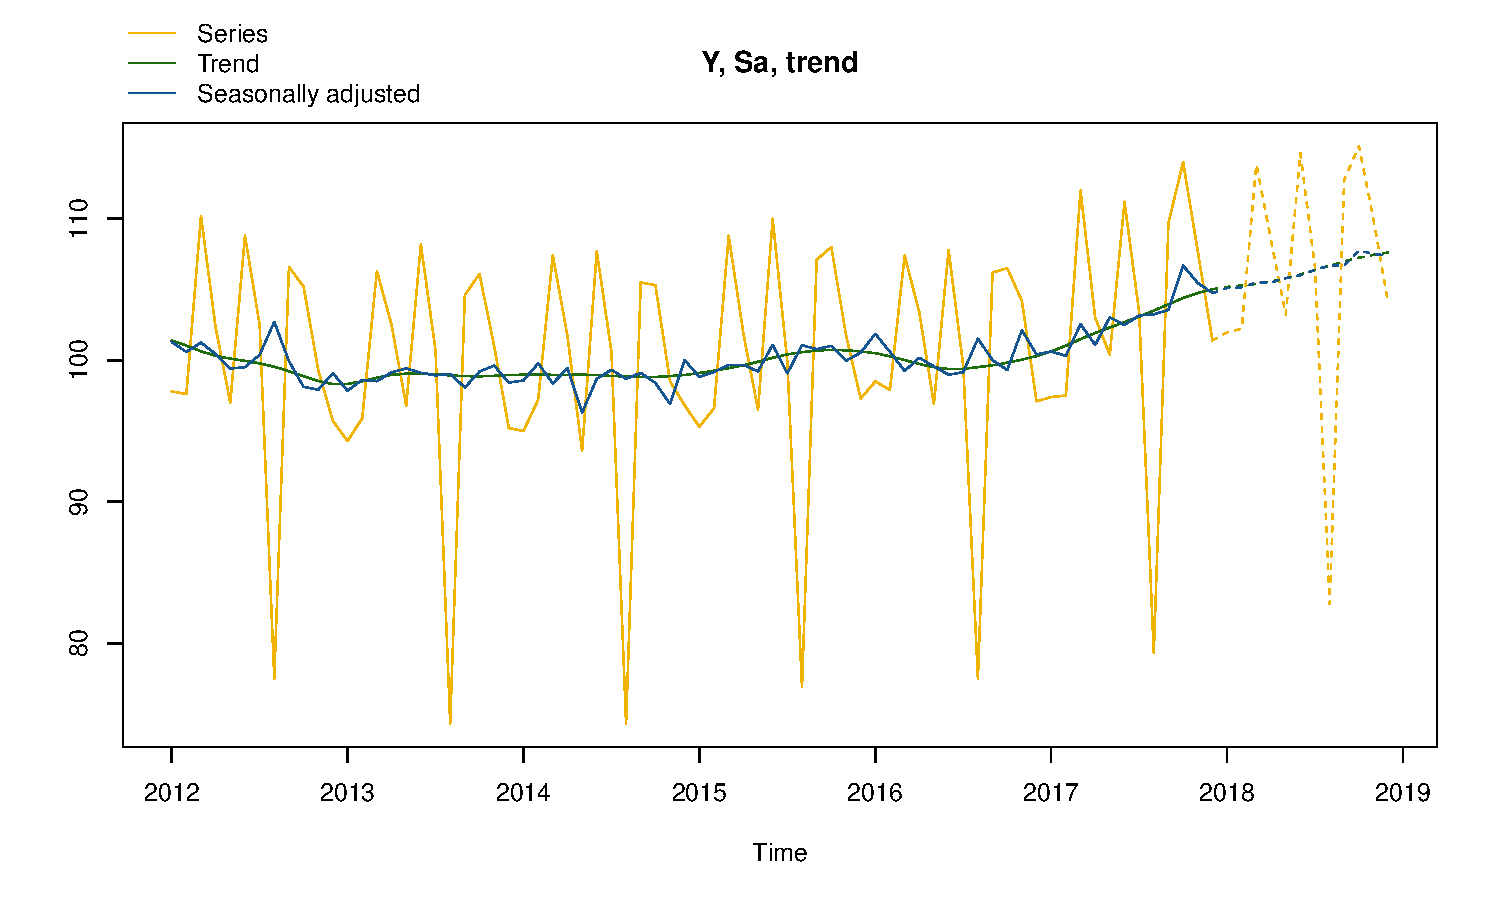
\includegraphics{img/markdown-unnamed-chunk-11-1.pdf}

\end{frame}

\begin{frame}[fragile]{Seasonal adjustment examples (7/7)}
\protect\hypertarget{seasonal-adjustment-examples-77}{}

\footnotesize

\begin{Shaded}
\begin{Highlighting}[]
\NormalTok{x13_mod}\OperatorTok{$}\NormalTok{diagnostics}
\end{Highlighting}
\end{Shaded}

\begin{verbatim}
##  Relative contribution of the components to the stationary
##  portion of the variance in the original series,
##  after the removal of the long term trend 
##  Trend computed by Hodrick-Prescott filter (cycle length = 8.0 years)
##            Component
##  Cycle         1.656
##  Seasonal     39.710
##  Irregular     0.369
##  TD & Hol.     0.000
##  Others       61.757
##  Total       103.492
## 
##  Combined test in the entire series 
##  Non parametric tests for stable seasonality
##                                                           P.value
##    Kruskall-Wallis test                                      0.000
##    Test for the presence of seasonality assuming stability   0.000
##    Evolutive seasonality test                                0.024
##  
##  Identifiable seasonality present
## 
##  Residual seasonality tests 
##                                       P.value
##  qs test on sa                          1.000
##  qs test on i                           1.000
##  f-test on sa (seasonal dummies)        0.985
##  f-test on i (seasonal dummies)         0.917
##  Residual seasonality (entire series)   0.991
##  Residual seasonality (last 3 years)    0.971
##  f-test on sa (td)                      0.001
##  f-test on i (td)                       0.006
\end{verbatim}

\end{frame}

\hypertarget{manipulate-workspaces}{%
\subsection{Manipulate workspaces}\label{manipulate-workspaces}}

\begin{frame}[fragile]{Export a workspace}
\protect\hypertarget{export-a-workspace}{}

\footnotesize

\begin{Shaded}
\begin{Highlighting}[]
\NormalTok{wk <-}\StringTok{ }\KeywordTok{new_workspace}\NormalTok{()}
\KeywordTok{new_multiprocessing}\NormalTok{(wk, }\DataTypeTok{name =} \StringTok{"MP-1"}\NormalTok{)}
\KeywordTok{add_sa_item}\NormalTok{(wk, }\DataTypeTok{multiprocessing =} \StringTok{"MP-1"}\NormalTok{,}
            \DataTypeTok{sa_obj =}\NormalTok{ x13_mod, }\DataTypeTok{name =}  \StringTok{"SA with X13 model 1 "}\NormalTok{)}
\KeywordTok{add_sa_item}\NormalTok{(wk, }\DataTypeTok{multiprocessing =}  \StringTok{"MP-1"}\NormalTok{,}
            \DataTypeTok{sa_obj =}\NormalTok{ ts_mod, }\DataTypeTok{name =} \StringTok{"SA with TramoSeats model 1"}\NormalTok{)}
\KeywordTok{save_workspace}\NormalTok{(wk, }\StringTok{"workspace.xml"}\NormalTok{)}
\end{Highlighting}
\end{Shaded}

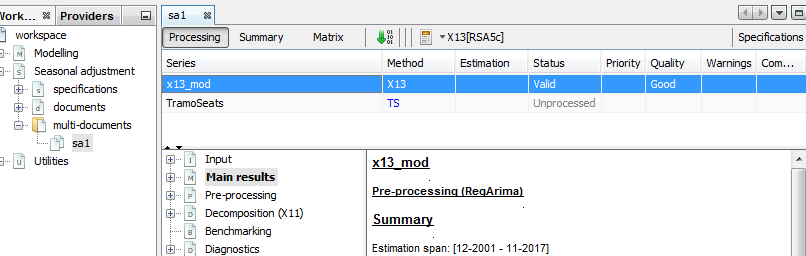
\includegraphics{img/workspace.png}

\end{frame}

\begin{frame}[fragile]{Import a workspace (1/3)}
\protect\hypertarget{import-a-workspace-13}{}

\footnotesize

\begin{Shaded}
\begin{Highlighting}[]
\NormalTok{wk <-}\StringTok{ }\KeywordTok{load_workspace}\NormalTok{(}\StringTok{"workspace.xml"}\NormalTok{)}
\KeywordTok{get_ts}\NormalTok{(wk)}
\end{Highlighting}
\end{Shaded}

\begin{verbatim}
## $`MP-1`
## $`MP-1`$`SA with X13 model 1 `
##        Jan   Feb   Mar   Apr   May   Jun   Jul   Aug   Sep   Oct   Nov
## 1990  90.5  92.6 101.9  95.2  92.1 103.3  91.8  65.5  99.0 102.8  94.3
## 1991  90.9  89.6  99.9  93.3  88.3 103.0  89.7  65.1  98.2 100.8  95.8
## 1992  89.4  89.0  99.5  93.0  89.1 101.3  89.4  64.1  94.9  98.6  92.2
## 1993  85.3  84.3  93.2  87.8  83.5  95.4  86.2  60.1  92.1  95.8  88.1
## 1994  84.9  84.0  94.1  90.1  86.8 100.4  90.8  64.5  96.8 101.0  96.6
## 1995  90.4  90.5 100.4  94.5  89.7 103.7  93.8  65.5  99.7 101.8  94.6
## 1996  90.3  88.8 100.7  93.8  91.2 104.4  92.3  67.2 100.2 102.3  96.9
## 1997  90.5  91.6 104.0  99.7  93.9 108.8  98.2  73.4 105.8 111.8 102.4
## 1998  99.2  99.0 109.4 103.0 100.7 114.8 104.9  73.3 109.6 112.7 105.9
## 1999 100.5  98.6 111.8 104.3 101.3 117.4 106.6  74.9 113.4 118.2 110.9
## 2000 104.8 104.9 118.9 110.2 108.0 122.5 111.8  80.5 117.5 121.7 114.3
## 2001 108.8 109.2 123.7 111.8 108.4 124.7 111.1  84.2 117.8 121.0 111.6
## 2002 106.6 107.0 121.4 112.8 106.4 122.2 109.7  82.3 117.1 118.7 113.0
## 2003 105.4 105.7 120.1 111.1 102.8 118.3 108.8  78.7 115.9 119.9 110.8
## 2004 105.8 107.0 120.0 112.1 105.8 123.6 112.0  78.4 120.0 122.0 112.0
## 2005 109.1 106.7 117.9 113.5 106.8 122.3 110.3  80.0 121.4 118.4 115.2
## 2006 107.3 106.3 121.9 112.5 110.8 126.7 112.5  82.5 122.2 121.9 113.7
## 2007 109.5 110.0 123.8 114.2 112.6 127.0 115.2  85.7 121.2 124.7 115.2
## 2008 111.4 112.2 123.0 116.8 108.4 122.1 112.6  81.9 117.3 116.3 102.4
## 2009  91.7  90.4 100.1  93.2  91.4 105.5  96.8  71.6 104.5 104.8  99.3
## 2010  93.7  93.5 106.8  99.9  96.9 108.9 101.7  73.2 107.2 108.2 102.5
## 2011 100.4 102.0 112.0 103.7 102.9 111.3 105.0  76.6 108.4 109.7 106.0
## 2012  97.8  97.6 110.2 102.3  97.0 108.8 102.5  77.5 106.6 105.2  99.3
## 2013  94.3  95.9 106.3 102.5  96.8 108.2 100.7  74.3 104.6 106.1 101.0
## 2014  95.0  97.2 107.4 101.7  93.6 107.7 100.6  74.3 105.5 105.3  98.5
## 2015  95.3  96.6 108.8 101.9  96.5 110.0  99.9  76.9 107.1 108.0 101.8
## 2016  98.5  97.9 107.4 103.4  96.9 107.8  99.6  77.5 106.2 106.5 104.2
## 2017  97.4  97.5 112.0 103.0 100.4 111.2 103.4  79.3 109.7 114.0 107.7
##        Dec
## 1990  93.1
## 1991  93.2
## 1992  90.5
## 1993  88.3
## 1994  96.3
## 1995  98.1
## 1996  97.2
## 1997 105.4
## 1998 105.1
## 1999 109.8
## 2000 115.5
## 2001 109.2
## 2002 106.4
## 2003 107.9
## 2004 108.4
## 2005 109.8
## 2006 111.7
## 2007 111.0
## 2008  97.8
## 2009  92.9
## 2010  97.9
## 2011  98.4
## 2012  95.7
## 2013  95.2
## 2014  96.8
## 2015  97.3
## 2016  97.1
## 2017 101.4
## 
## $`MP-1`$`SA with TramoSeats model 1`
##        Jan   Feb   Mar   Apr   May   Jun   Jul   Aug   Sep   Oct   Nov
## 1990  90.5  92.6 101.9  95.2  92.1 103.3  91.8  65.5  99.0 102.8  94.3
## 1991  90.9  89.6  99.9  93.3  88.3 103.0  89.7  65.1  98.2 100.8  95.8
## 1992  89.4  89.0  99.5  93.0  89.1 101.3  89.4  64.1  94.9  98.6  92.2
## 1993  85.3  84.3  93.2  87.8  83.5  95.4  86.2  60.1  92.1  95.8  88.1
## 1994  84.9  84.0  94.1  90.1  86.8 100.4  90.8  64.5  96.8 101.0  96.6
## 1995  90.4  90.5 100.4  94.5  89.7 103.7  93.8  65.5  99.7 101.8  94.6
## 1996  90.3  88.8 100.7  93.8  91.2 104.4  92.3  67.2 100.2 102.3  96.9
## 1997  90.5  91.6 104.0  99.7  93.9 108.8  98.2  73.4 105.8 111.8 102.4
## 1998  99.2  99.0 109.4 103.0 100.7 114.8 104.9  73.3 109.6 112.7 105.9
## 1999 100.5  98.6 111.8 104.3 101.3 117.4 106.6  74.9 113.4 118.2 110.9
## 2000 104.8 104.9 118.9 110.2 108.0 122.5 111.8  80.5 117.5 121.7 114.3
## 2001 108.8 109.2 123.7 111.8 108.4 124.7 111.1  84.2 117.8 121.0 111.6
## 2002 106.6 107.0 121.4 112.8 106.4 122.2 109.7  82.3 117.1 118.7 113.0
## 2003 105.4 105.7 120.1 111.1 102.8 118.3 108.8  78.7 115.9 119.9 110.8
## 2004 105.8 107.0 120.0 112.1 105.8 123.6 112.0  78.4 120.0 122.0 112.0
## 2005 109.1 106.7 117.9 113.5 106.8 122.3 110.3  80.0 121.4 118.4 115.2
## 2006 107.3 106.3 121.9 112.5 110.8 126.7 112.5  82.5 122.2 121.9 113.7
## 2007 109.5 110.0 123.8 114.2 112.6 127.0 115.2  85.7 121.2 124.7 115.2
## 2008 111.4 112.2 123.0 116.8 108.4 122.1 112.6  81.9 117.3 116.3 102.4
## 2009  91.7  90.4 100.1  93.2  91.4 105.5  96.8  71.6 104.5 104.8  99.3
## 2010  93.7  93.5 106.8  99.9  96.9 108.9 101.7  73.2 107.2 108.2 102.5
## 2011 100.4 102.0 112.0 103.7 102.9 111.3 105.0  76.6 108.4 109.7 106.0
## 2012  97.8  97.6 110.2 102.3  97.0 108.8 102.5  77.5 106.6 105.2  99.3
## 2013  94.3  95.9 106.3 102.5  96.8 108.2 100.7  74.3 104.6 106.1 101.0
## 2014  95.0  97.2 107.4 101.7  93.6 107.7 100.6  74.3 105.5 105.3  98.5
## 2015  95.3  96.6 108.8 101.9  96.5 110.0  99.9  76.9 107.1 108.0 101.8
## 2016  98.5  97.9 107.4 103.4  96.9 107.8  99.6  77.5 106.2 106.5 104.2
## 2017  97.4  97.5 112.0 103.0 100.4 111.2 103.4  79.3 109.7 114.0 107.7
##        Dec
## 1990  93.1
## 1991  93.2
## 1992  90.5
## 1993  88.3
## 1994  96.3
## 1995  98.1
## 1996  97.2
## 1997 105.4
## 1998 105.1
## 1999 109.8
## 2000 115.5
## 2001 109.2
## 2002 106.4
## 2003 107.9
## 2004 108.4
## 2005 109.8
## 2006 111.7
## 2007 111.0
## 2008  97.8
## 2009  92.9
## 2010  97.9
## 2011  98.4
## 2012  95.7
## 2013  95.2
## 2014  96.8
## 2015  97.3
## 2016  97.1
## 2017 101.4
\end{verbatim}

\end{frame}

\begin{frame}{Import a workspace (2/3)}
\protect\hypertarget{import-a-workspace-23}{}

\animategraphics[loop, autoplay, width=\linewidth]{7}{img/gif/import_model/}{1}{97}

\end{frame}

\begin{frame}[fragile]{Import a workspace (3/3)}
\protect\hypertarget{import-a-workspace-33}{}

\footnotesize

\begin{Shaded}
\begin{Highlighting}[]
\KeywordTok{compute}\NormalTok{(wk) }\CommentTok{# Important to get the Sa model}
\NormalTok{models <-}\StringTok{ }\KeywordTok{get_model}\NormalTok{(wk) }\CommentTok{# A progress bar is printed by default}
\end{Highlighting}
\end{Shaded}

\begin{verbatim}
## Multiprocessing 1 on 1:
## 
  |                                                                       
  |                                                                 |   0%
  |                                                                       
  |================================                                 |  50%
  |                                                                       
  |=================================================================| 100%
\end{verbatim}

\begin{Shaded}
\begin{Highlighting}[]
\CommentTok{# To extract only one model}
\NormalTok{mp <-}\StringTok{ }\KeywordTok{get_object}\NormalTok{(wk, }\DecValTok{1}\NormalTok{)}
\KeywordTok{count}\NormalTok{(mp)}
\end{Highlighting}
\end{Shaded}

\begin{verbatim}
## [1] 2
\end{verbatim}

\begin{Shaded}
\begin{Highlighting}[]
\NormalTok{sa2 <-}\StringTok{ }\KeywordTok{get_object}\NormalTok{(mp,}\DecValTok{2}\NormalTok{)}
\KeywordTok{get_name}\NormalTok{(sa2)}
\end{Highlighting}
\end{Shaded}

\begin{verbatim}
## [1] "SA with TramoSeats model 1"
\end{verbatim}

\begin{Shaded}
\begin{Highlighting}[]
\NormalTok{mod <-}\StringTok{ }\KeywordTok{get_model}\NormalTok{(wk, sa2)}
\end{Highlighting}
\end{Shaded}

\begin{verbatim}
## Multiprocessing 1 on 1:
## 
  |                                                                       
  |                                                                 |   0%
  |                                                                       
  |================================                                 |  50%
  |                                                                       
  |=================================================================| 100%
\end{verbatim}

\end{frame}

\hypertarget{installation-and-future-development}{%
\subsection{Installation and future
development}\label{installation-and-future-development}}

\begin{frame}[fragile]{How to install the package?}
\protect\hypertarget{how-to-install-the-package}{}

The package is available on GitHub:
\url{https://github.com/jdemetra/rjdemetra}

It has also it's own website:
\url{https://jdemetra.github.io/rjdemetra/}

It package can be installed from CRAN:

\begin{Shaded}
\begin{Highlighting}[]
\KeywordTok{install.packages}\NormalTok{(}\StringTok{"RJDemetra"}\NormalTok{)}
\end{Highlighting}
\end{Shaded}

Or from github (development version):

\begin{Shaded}
\begin{Highlighting}[]
\NormalTok{devtools}\OperatorTok{::}\KeywordTok{install_github}\NormalTok{(}\StringTok{"jdemetra/rjdemetra"}\NormalTok{)}
\end{Highlighting}
\end{Shaded}

\bcinfo To install it you need Java8: in case you don't, install a
portable version of Java8 and set the \texttt{JAVA\_HOME} path.

\end{frame}

\hypertarget{future-developments}{%
\subsection{Future developments}\label{future-developments}}

\begin{frame}{What's next? \bcpanchant (1/2)}
\protect\hypertarget{whats-next-12}{}

Documentation:

\begin{itemize}
\item
  Vignette/article for the Journal of Statistical Software
\item
  Guide to install the package with portable version of Java (when you
  don't have administrator rights)
\item
  Cheat sheet
\end{itemize}

\end{frame}

\begin{frame}{What's next? \bcpanchant (2/2)}
\protect\hypertarget{whats-next-22}{}

Package:

\begin{itemize}
\item
  Get only the Java object of a SA (to reduce computation/customize the
  output)
\item
  Possibility to used user-defined calendar regressors (currently: only
  user-defined regressors)
\item
  Function to ``refresh'' the model (JD+ 3.0.0)
\end{itemize}

\end{frame}

\begin{frame}[fragile]{Why and how use RJDemetra?}
\protect\hypertarget{why-and-how-use-rjdemetra}{}


\includegraphics[height = 1.5cm]{img/rjdqa_logo.png} A package for
quality assessment for seasonal adjustment. It implements:

\begin{itemize}
\item
  Statistics Canada Dashboard (to provide a snapshot of an individual
  series at a point in time and points out some possible problems)
\item
  Insee quality report matrix (used to help the analyst during
  production to prioritize the models to check)
\end{itemize}

\(\rightarrow\) See the
\href{https://ec.europa.eu/eurostat/web/products-manuals-and-guidelines/-/KS-GQ-18-001?inheritRedirect=true}{Seasonal
Adjustment handbook}

Available on github \url{https://github.com/AQLT/rjdqa}, still in
development (only works for X13 models and no documentation yet)

Example of the dashboard:

\begin{Shaded}
\begin{Highlighting}[]
\KeywordTok{library}\NormalTok{(rjdqa)}
\KeywordTok{plot}\NormalTok{(}\KeywordTok{sa_dashboard}\NormalTok{(x13_mod))}
\end{Highlighting}
\end{Shaded}

\end{frame}

\hypertarget{statistics-canada-dashboard}{%
\subsection{Statistics Canada
dashboard}\label{statistics-canada-dashboard}}

\begin{frame}[fragile]{Example of the dashboard (1/2)}
\protect\hypertarget{example-of-the-dashboard-12}{}

\footnotesize

\begin{verbatim}
## 
## Attaching package: 'rjdqa'
\end{verbatim}

\begin{verbatim}
## The following object is masked _by_ '.GlobalEnv':
## 
##     myseries
\end{verbatim}

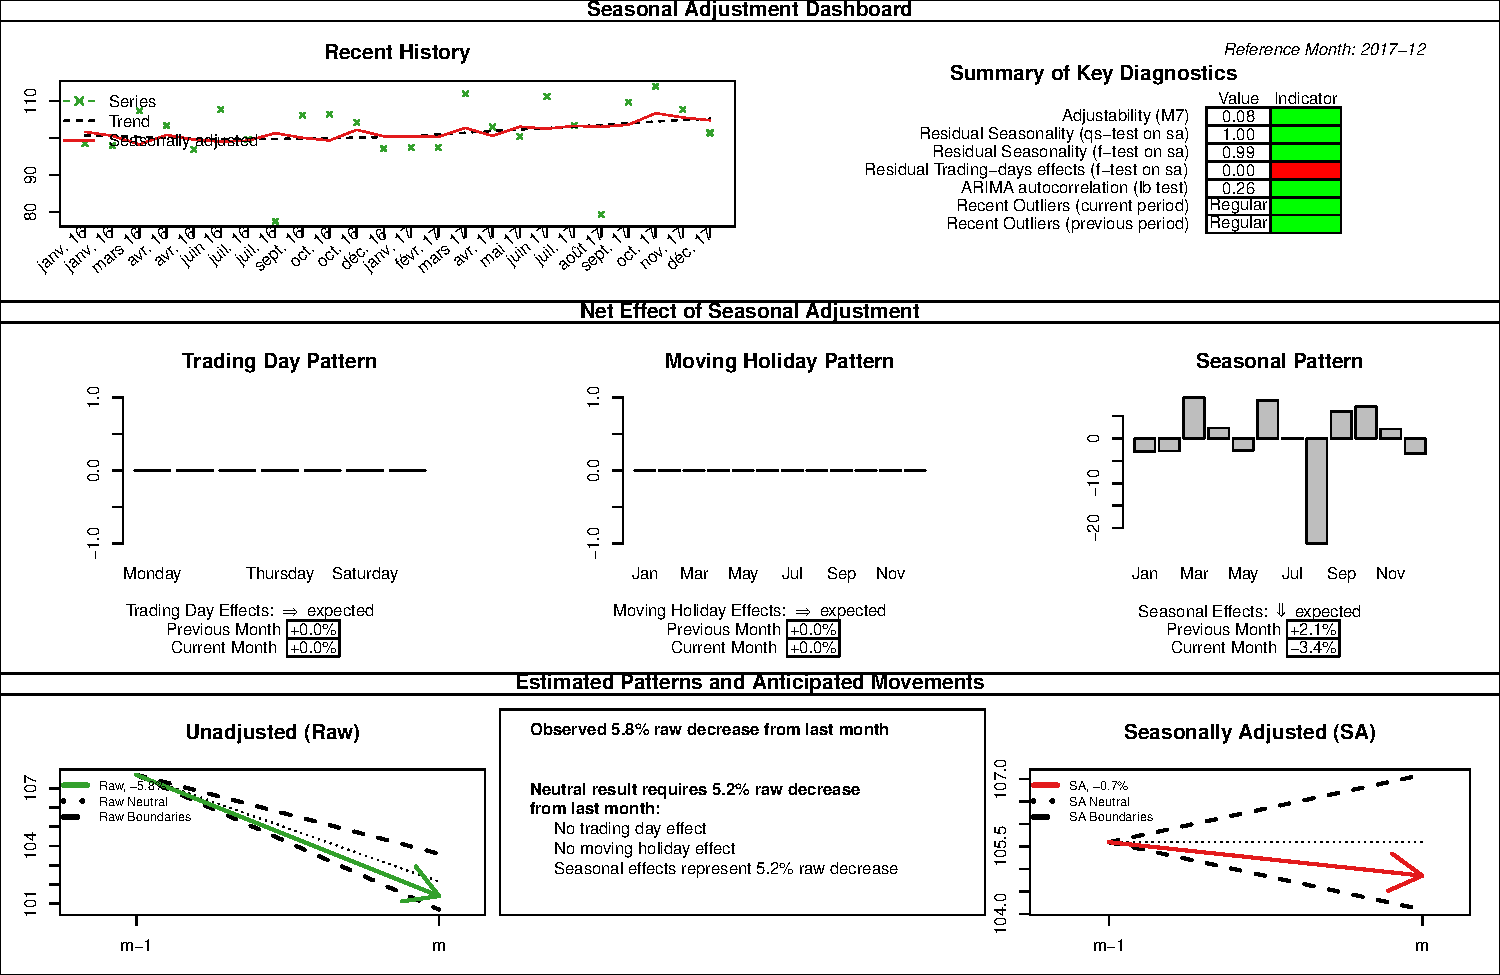
\includegraphics{img/markdown-unnamed-chunk-19-1.pdf}

\end{frame}

\begin{frame}{Example of the dashboard (2/2)}
\protect\hypertarget{example-of-the-dashboard-22}{}

\begin{enumerate}
\item
  \textbf{Recent History of Series}: plot of the raw series, the SA
  series and the trend for the most recent periods. It is intended to
  identify trend direction, overall volatility and obvious outliers
\item
  \textbf{Summary of Key Diagnostics}: key diagnostics as residual
  seasonality, recent and recurring outliers, moving seasonality, ARIMA
  model autocorrelation
\item
  \textbf{Estimated Patterns and Anticipated Movements}: estimated
  trading day, moving holiday and seasonal pattern (rescaled in additive
  decomposition to represent relative level)
\item
  \textbf{Net Effect of Seasonal Adjustment}: movement in the raw
  series, compared to typical ranges centered around ``neutral'' value
  (when \(SA_t = SA_{t-1}\))
\end{enumerate}

\end{frame}

\end{document}
